\section{Methodologies}
\subsection{U-net-based Wildfire Detection}
Considering the rapidly shape changing and blurred edge of smoke, U-net is advocated in this research because of its fantastic performance in medical image processing fields. With the original image information or the restored images from UAV in forest, U-net could be deployed for wildfire smoke or flame segmentation. The U-net structure could be illustrated in Fig.~\ref{fig:figureUnetmodel}.
\begin{figure}[ht]
    \centering
    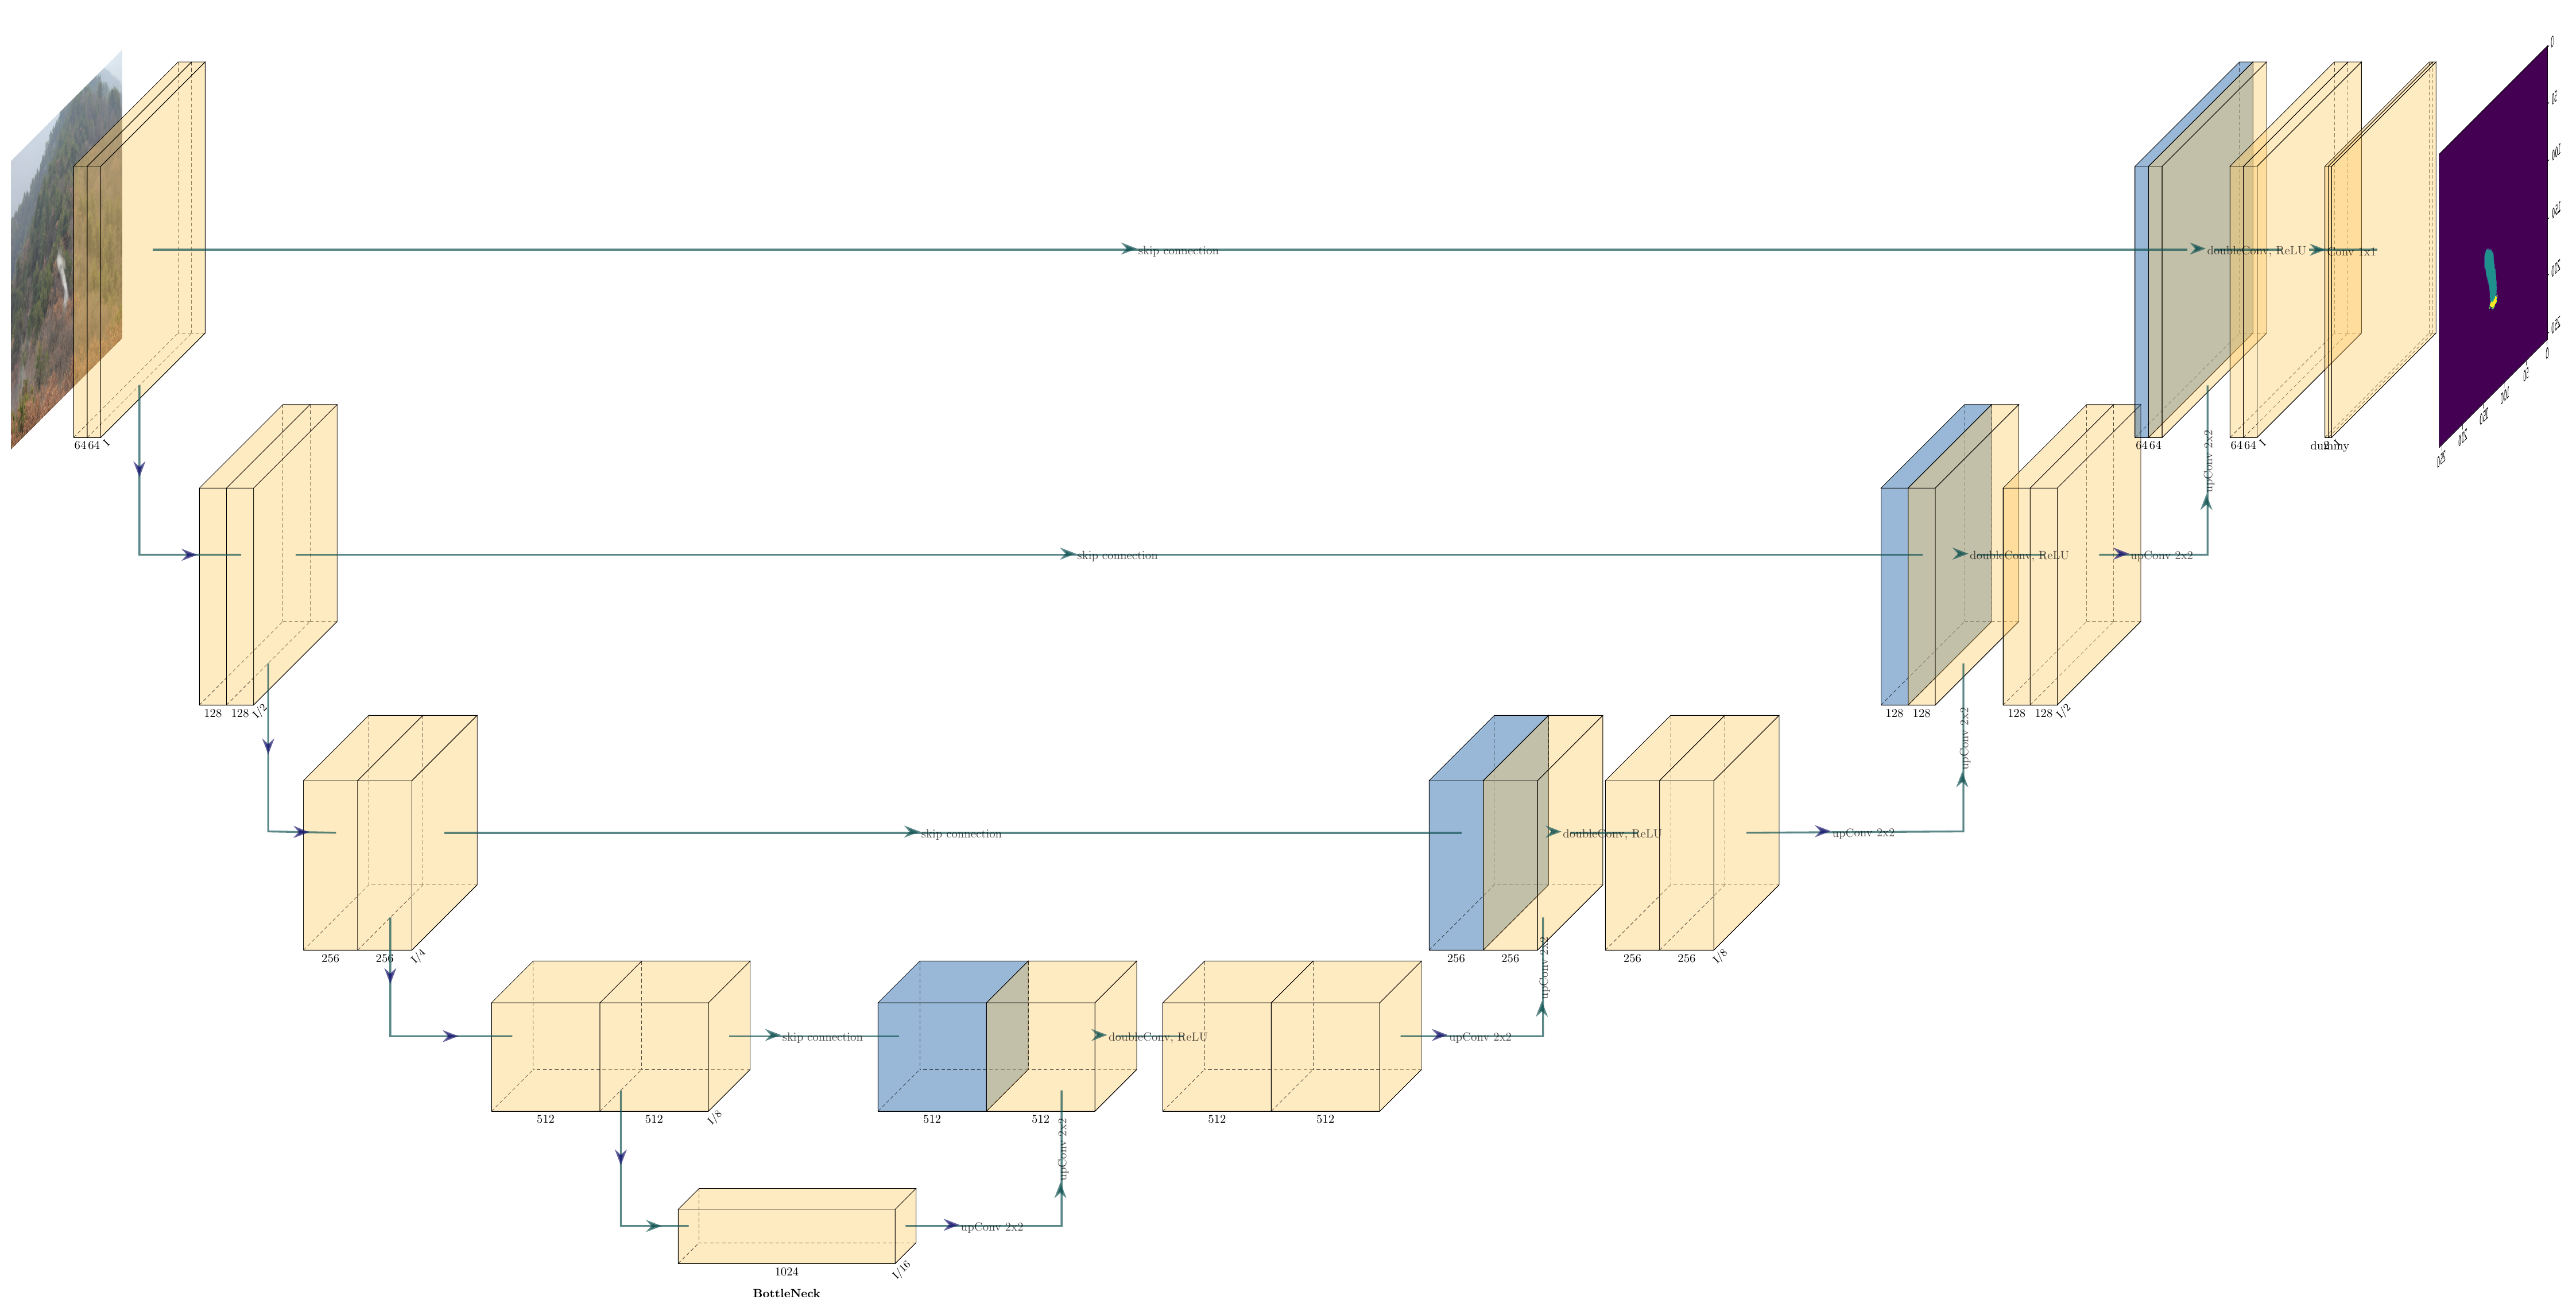
\includegraphics[height=60mm]{figs/figureUnetmodel.png}
    \caption{Brief structure of the U-net deployed on DJI M300 for the first time experiment}
    \label{fig:figureUnetmodel}
\end{figure}\par
The structure shown in Fig.~\ref{fig:figureUnetmodel} is the one which based on ResNet18 and the first time experiment demonstrated that it could be deployed on-board with the support of tensor2trt to get FPS of 5 as dealing with original images. However, the segmentation accuracy still need to be improved and the size of this model could be decreased when using the concept of SqueezeNet. At ground work station, the deployment environment is not that serious as on-board, but the segmentation accuracy should be higher than on-board ones. Therefore, higher level residual networks could also be considered to build a U-net for wildfire smoke and flame segmentation. These apply-able network structures are illustrated in Table.~\ref{table: fcnforunet}.
\begin{table}[!ht]
    \centering
    \caption{Residual network structures for building the U-net for wildfire detection}
    \label{table: fcnforunet}
        \resizebox{\textwidth}{!}{
        \begin{tabular}{c c c c c c c}
        \toprule
        Layers &
        Output &
        18-layers&
        34-layers&
        50-layers&
        101-layers&
        152-layers\\
        \midrule
        \rowcolor{mygray}
        Conv1 &
        $112\times 112$&
        \multicolumn{5}{c}{
        \text{kernel size} = $7\times7$, \text{out channel} = 64, \text{stride} = 2, \text{padding} = 3
        } \\
        \rowcolor{mygray}
        Pool1 &
        $112\times 112$&
        \multicolumn{5}{c}{
        \text{kernel size} = $3\times3$, \text{type} = \text{max pool}, \text{stride} = 2
        }\\
        Conv2x &
        $56\times 56$&
        \left[
        \begin{array}{c}
            3\times 3, 64\\ 3\times 3, 64
        \end{array}
        \right] \times 2 &
        \left[
        \begin{array}{c}
            3\times 3, 64 \\ 3\times 3, 64
        \end{array}
        \right] \times 3 &
        \left[
        \begin{array}{c}
            1\times 1, 64 \\ 3\times 3, 64\\ 1\times 1, 256\\
        \end{array}
        \right] \times 3 &
        \left[
        \begin{array}{c}
            1\times 1, 64 \\ 3\times 3, 64\\ 1\times 1, 256
        \end{array}
        \right] \times 3 &
        \left[
        \begin{array}{c}
            1\times 1, 64 \\ 3\times 3, 64\\ 1\times 1, 256
        \end{array}
        \right] \times 3\\
        
        \rowcolor{mygray}
        Conv3x&
        28\times 28&
        \left[
        \begin{array}{c}
             3\times 3, 128\\ 3\times 3, 128
        \end{array}
        \right] \times 2 &
        \left[
        \begin{array}{c}
            3\times 3, 128 \\ 3\times 3, 128
        \end{array}
        \right] \times 4 &
        \left[
        \begin{array}{c}
            1\times 1, 128 \\ 3\times 3, 128\\ 1\times 1, 512
        \end{array}
        \right] \times 4 &
        \left[
        \begin{array}{c}
            1\times 1, 128 \\ 3\times 3, 128\\ 1\times 1, 512
        \end{array}
        \right] \times 4 &
        \left[
        \begin{array}{c}
            1\times 1, 128 \\ 3\times 3, 128\\ 1\times 1, 512
        \end{array}
        \right] \times 8 &\\
        Conv4x &
        14\times14&
        \left[
        \begin{array}{c}
            3\times 3, 256 \\ 3\times 3, 256\\
        \end{array}
        \right] \times 2 &
        \left[
        \begin{array}{c}
            3\times 3, 256 \\ 3\times 3, 256\\
        \end{array}
        \right] \times 6 &
        \left[
        \begin{array}{c}
            1\times 1, 256 \\ 3\times 3, 256\\ 1\times 1, 1024
        \end{array}
        \right] \times 6 &
        \left[
        \begin{array}{c}
            1\times 1, 256 \\ 3\times 3, 256\\ 1\times 1, 1024
        \end{array}
        \right] \times 23 &
        \left[
        \begin{array}{c}
            1\times 1, 256 \\ 3\times 3, 256\\ 1\times 1, 1024
        \end{array}
        \right] \times 36 &\\
        \rowcolor{mygray}
        Conv5x&
        7\times7&
        \left[
        \begin{array}{c}
            3\times 3, 512 \\ 3\times 3, 512
        \end{array}
        \right] \times 2 &
        \left[
        \begin{array}{c}
            3\times 3, 512 \\ 3\times 3, 512
        \end{array}
        \right] \times 3 &
        \left[
        \begin{array}{c}
            1\times 1, 512 \\ 3\times 3, 512\\ 1\times 1, 2048
        \end{array}
        \right] \times 3 &
        \left[
        \begin{array}{c}
            1\times 1, 512 \\ 3\times 3, 512\\ 1\times 1, 2048
        \end{array}
        \right] \times 3 &
        \left[
        \begin{array}{c}
            1\times 1, 512 \\ 3\times 3, 512\\ 1\times 1, 2048
        \end{array}
        \right] \times 3\\
        \bottomrule
        \end{tabular}}
\end{table}
\subsection{Squeeze Model}
To deploy the U-net on-board with less computational resource demands, the squeeze model is consider for developing the ResNet18-based U-net into a light model. Attention mechanism is also able to be developed to design attention gate at the skip connection parts of U-net to filter higher value features before up-sampling parts to increase the feature learning efficiency.\par
On the other hand, attention mechanism could not only be applied to develop the U-net for wildfire detection. It could also be helpful in building the NN-based prediction model for the fire fronts spreading. Such concept is also stated at the conclusion part of \cite{peng2019real}. Therefore, the squeeze model and attention mechanism are going to be described as follow.
\subsubsection{Squeeze Model}
Fig.~\ref{fig:figureSqueezemodel} shows the brief structure of the squeeze and unsqueeze model.

\subsubsection{Attention Mechanism}

\subsection{GAN-based Wildfire Image Restoration}
Considering the signal missing and disturbance as UAV capturing image information in wide forest environment. Generative adversarial network (GAN)-based image restoration is going to be designed. GAN could be separate into two parts: generator ($G$) and discriminator ($D$). The generating continues until the discriminator could not distinguish which is the target or which is the generated image, it is considered converged.\par
It should be noticed that, such strategy should only be applied in very serious forest environment and extreme situation. Because the GAN should be deployed on-board, where the computation resource distribution will be very challenging as other schemes are working to support the wildfire detection. And strictly, the restored information are not the real original information, there is risk that the restored image might misleading the segmentation of smoke edge.
Commonly, the GAN structure could be illustrated in Fig.~\ref{fig:figureGANmodel}.
\begin{figure}[ht]
    \centering
    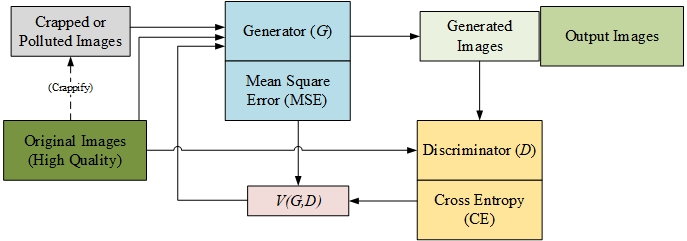
\includegraphics[height=40mm]{figs/figureGANmodel.jpg}
    \caption{Brief GAN structure as training process}
    \label{fig:figureGANmodel}
\end{figure}
It could be considered that, GAN is to balance the loss of $G$ and $D$. Mean squared error (MSE) could be applied as the main loss function of GAN. In the training process, MSE is to compare the pixel values of generated image and high quality image, it can be written in a form of Eq.~\ref{eq: MSE}.
\begin{equation}
\text{MSE}(y, \hat y) =
\frac{\sum_{i=0}^N (y_i-\hat y_i)^2}{N}
\label{eq: MSE}
\end{equation}
Value function $V(G, D)$ could be applied as Eq.~\ref{eq: valueloss} to describe the balance process of GAN.
\begin{equation}
\min_G\max_D V(G,D)=
\mathbf{E}_{x~p_{data}{x}}[\log D(x)]+
\mathbf{E}_{z~p_z{z}}[log(1-D(G(z)))]
\label{eq: valueloss}
\end{equation}
\subsection{Cellular Model for Wildfire Prediction}
\subsection{VOT-based Wildfire Tracking}






